\section{Alzheimer’s disease and early diagnosis}

Alzheimer's disease (AD) is the most common cause of dementia and one of the major clinical challenges associated with population ageing. It is a progressive neurodegenerative disorder in which cognitive and functional decline usually emerge after a long period of underlying biological change. Clinically, AD is commonly associated with impairment in episodic memory, followed by decline in additional cognitive domains and progressive loss of independence. However, the current understanding of AD is no longer limited to the stage in which dementia is clinically apparent. The disease is increasingly interpreted as a long biological process that precedes, and eventually may lead to, the clinical syndrome of dementia \cite{scheltens2021alzheimer,jack2018nia}.

From a pathological perspective, AD is characterized by the accumulation of amyloid-\(\beta\) plaques and tau neurofibrillary tangles, together with synaptic dysfunction, neuronal injury, and neurodegeneration. These processes do not occur as a single event, nor do they necessarily coincide with the first observable cognitive symptoms. Instead, AD develops across a continuum in which molecular and cellular abnormalities may be detectable before dementia-level impairment becomes evident \cite{scheltens2021alzheimer,sperling2011preclinical}. This temporal separation between biological disease and clinical manifestation is central to modern AD research, because it makes early detection and disease staging conceptually different from the traditional diagnosis of dementia.

A major conceptual shift in the field has been the transition from a purely clinical definition of AD to a biological definition. The 2018 NIA-AA Research Framework explicitly defines AD by its underlying pathologic processes rather than by the presence of clinical symptoms alone \cite{jack2018nia}. In this framework, cognitive status and biological disease status are separated: an individual may show biomarker evidence of AD pathology while remaining cognitively unimpaired, or may present cognitive impairment whose underlying cause requires biological confirmation. The framework organizes AD biomarkers according to the AT(N) system, where ``A'' refers to amyloid-\(\beta\) deposition, ``T'' to pathologic tau, and ``N'' to neurodegeneration or neuronal injury \cite{jack2018nia}.

The revised Alzheimer's Association criteria further reinforce the biological framing of AD and reflect the increasing role of biomarkers in diagnosis and staging \cite{jack2024revised}. This shift is especially important because it clarifies that AD should not be equated automatically with dementia. Dementia is a clinical syndrome, whereas AD is a biological disease process that can be present across different clinical stages. At the same time, many public biomedical datasets still use diagnostic labels such as AD, mild cognitive impairment (MCI), and cognitively normal control, often without complete biomarker confirmation. Therefore, in computational studies, these labels should be interpreted as practical supervised learning targets, not as perfect representations of underlying biological disease states.

This distinction is directly relevant to the present thesis. The classification task considered here focuses on distinguishing AD from MCI using blood gene expression data. This is not equivalent to separating diseased individuals from healthy controls. Instead, it involves diagnostic categories that may lie close to one another along the clinical and biological continuum of AD. For this reason, the task requires a cautious interpretation: a model trained on diagnostic labels may capture differences related to disease stage, symptom severity, systemic biological alterations, or dataset-specific effects, rather than a direct and isolated signature of AD pathology.

\chapter{Problem}
\label{ch:problem}

\section{Problem formulation and research setting}
\label{sec:problem-formulation}

The central problem addressed in this thesis is the classification of Alzheimer's disease (AD)-related clinical groups from peripheral blood gene expression data. More specifically, the thesis focuses on the distinction between subjects diagnosed with AD dementia and subjects diagnosed with mild cognitive impairment (MCI). This choice is deliberate. In much of the blood-transcriptomics literature, the most common benchmark is AD versus cognitively normal controls (CTL). That comparison is useful, but it is also a comparatively easier disease-versus-control setting. The clinically more informative question for this work is whether blood expression profiles contain enough signal to distinguish AD from MCI, two groups that are closer along the clinical continuum of cognitive decline.

This framing follows from the biological and clinical discussion introduced in Chapter~1. AD is no longer understood only as the dementia stage of disease. It is a biological process that can precede clinical dementia by many years, and MCI may represent a symptomatic intermediate stage for some individuals \cite{jack2018nia,albert2011diagnosis}. However, MCI is not equivalent to prodromal AD in every case. It is a heterogeneous clinical category: some subjects may later progress to AD dementia, some may remain stable, and some may have impairment driven by other mechanisms \cite{petersen2004mci}. Therefore, a supervised model trained to separate AD from MCI is not solving a simple healthy-versus-diseased problem. It is learning from two diagnostic labels that are close, noisy, and only partially aligned with the underlying biological disease process.

The labels used in this thesis must therefore be interpreted with caution. They are clinical categories available in public datasets, not direct measurements of amyloid deposition, tau pathology, neuronal injury, or neurodegeneration. In the ideal diagnostic setting, clinical status would be integrated with biomarker evidence. In the present computational setting, the available labels provide a practical supervised learning target. This difference matters because it limits the interpretation of model performance. A classifier that separates AD and MCI may be capturing disease-stage differences, immune and inflammatory alterations, medication-related effects, comorbidities, age-related molecular variation, batch-specific structure, or a mixture of these factors. The thesis therefore treats classification performance as evidence of predictive signal in the available data, not as proof of a clinically deployable diagnostic biomarker.

The biomedical problem is translated into a supervised learning setting. Each subject is represented by a blood gene expression vector
\[
    \mathbf{x}_i \in \mathbb{R}^{p},
\]
where \(p\) denotes the number of retained gene-level expression features after preprocessing. For a dataset of \(n\) subjects, the complete expression matrix is
\[
    \mathbf{X} \in \mathbb{R}^{n \times p}.
\]
For the main task, each subject is assigned a binary label
\[
    y_i \in \{\mathrm{AD}, \mathrm{MCI}\}.
\]
The objective is to learn a predictive function
\[
    f: \mathbb{R}^{p} \rightarrow \{\mathrm{AD}, \mathrm{MCI}\}
\]
that maps each expression profile to its diagnostic label. The same formal structure is used for the reference task AD versus CTL, where the label set is
\[
    y_i \in \{\mathrm{AD}, \mathrm{CTL}\}.
\]

This formulation highlights two dimensions of difficulty. The first is biomedical. The difference between AD and MCI is expected to be subtle because both groups are clinically impaired or disease-adjacent, and MCI itself is biologically heterogeneous. The second is computational. Blood gene expression datasets are high-dimensional and small-sample: thousands of genes are measured for a few hundred subjects. This creates a high-dimensional, low-sample-size setting in which many features may appear discriminative by chance. In such a setting, model evaluation can easily become optimistic if feature selection, scaling, batch correction, or hyperparameter tuning are not handled inside the training procedure.

For this reason, the problem studied in the thesis is not only model selection. It is also a problem of experimental design. A method is useful only if it performs well under a protocol that limits leakage and evaluates generalization to held-out samples. This is especially important because several previous studies in the area report strong results under protocols that are difficult to compare directly. Some focus on AD versus CTL, some use multiclass CN/MCI/AD labels, some study MCI conversion rather than cross-sectional AD/MCI separation, and some apply preprocessing or feature engineering steps before validation. The present thesis therefore defines the task explicitly and uses a common evaluation protocol when comparing reproduced methods.

\section{Datasets}
\label{sec:datasets}

The experimental analysis is based on two public blood gene expression datasets from the Gene Expression Omnibus (GEO): GSE63060 and GSE63061 \cite{barrett2013geo}. Both datasets are associated with the AddNeuroMed study and contain peripheral blood samples from subjects labelled as AD, MCI, or CTL. These two datasets are frequently used in the literature on blood transcriptomics for AD, and for this reason they provide a useful basis for both model development and comparison with previous work.

The use of GSE63060 and GSE63061 is attractive for three reasons. First, they contain all three clinical groups needed to formulate AD/MCI and AD/CTL classification. Second, they are blood-based, which is aligned with the motivation of studying minimally invasive molecular signals. Third, they have been repeatedly used in prior studies, making them a natural reference point for state-of-the-art comparisons.

At the same time, the datasets are not a clean homogeneous benchmark. GSE63060 and GSE63061 were generated in two batches and on two versions of the Illumina HumanHT-12 microarray platform. GSE63060 is associated with the HumanHT-12 V3.0 platform, whereas GSE63061 is associated with the HumanHT-12 V4.0 platform. Therefore, the original probe spaces are not identical, and technical variation may be present even before any biological comparison is considered. In the pipeline used for this thesis, the datasets are harmonized to a common gene-level feature space. After preprocessing and alignment, the binary datasets used in the experiments contain 19,460 gene-level features.

Only samples with one of the target diagnostic labels were retained. Samples with missing, ambiguous, or non-target diagnostic information were excluded from the working cohort. After this filtering step, the full retained dataset contains 711 subjects: 284 AD, 189 MCI, and 238 CTL. The two binary tasks used in the thesis are derived from this retained cohort. The main AD versus MCI task contains 473 samples, while the reference AD versus CTL task contains 522 samples.

\begin{table}[htbp]
\centering
\caption{Working datasets used in this thesis. AD versus MCI is the main task; AD versus CTL is retained as a reference task for comparison with the literature.}
\label{tab:working-datasets}
\begin{tabular}{lccc}
\hline
Dataset & Classes & Samples & Features \\
\hline
Full retained cohort & AD, MCI, CTL & 711 & 19,460 \\
Main task & AD vs MCI & 473 & 19,460 \\
Reference task & AD vs CTL & 522 & 19,460 \\
\hline
\end{tabular}
\end{table}

The class distribution is moderately imbalanced. In the full retained cohort, AD is the largest class, CTL is intermediate, and MCI is the smallest class. In the main AD versus MCI task, the class distribution is 284 AD and 189 MCI. In the AD versus CTL reference task, the distribution is 284 AD and 238 CTL. This imbalance is not extreme, but it is important enough to affect metric choice. A model that predicts the majority class more reliably may obtain acceptable accuracy while still performing poorly on the minority class. This is one of the reasons why macro-F1 is used throughout the thesis.

\begin{table}[htbp]
\centering
\caption{Class distribution in the retained datasets.}
\label{tab:class-distribution}
\begin{tabular}{lccc}
\hline
Setting & AD & MCI & CTL \\
\hline
Full retained cohort & 284 & 189 & 238 \\
AD vs MCI & 284 & 189 & -- \\
AD vs CTL & 284 & -- & 238 \\
\hline
\end{tabular}
\end{table}

The available metadata include age, gender, ethnicity, clinical status, GEO accession, and dataset origin. These variables are important for describing the cohort and for identifying possible confounding factors. However, the thesis does not treat demographic metadata as the central predictive input. The main experimental question is whether transcriptomic profiles alone provide useful signal. Metadata are therefore discussed only insofar as they affect interpretation: age, sex, ethnicity, and dataset origin can all influence blood gene expression, and therefore they may contribute to apparent classification signal if not handled carefully.

The dataset origin variable is especially relevant because it identifies whether a sample comes from GSE63060 or GSE63061. This variable is not a biological label, but it can be correlated with technical effects. A classifier that learns to separate datasets rather than disease states would be misleading. For this reason, the evaluation protocol must make the batch structure visible. Internal random splits can be useful, but they are not sufficient on their own. Batch-holdout or cross-dataset tests are more informative because they evaluate whether a learned pattern survives a shift between dataset batches.

In summary, GSE63060 and GSE63061 provide a suitable but challenging data source for this thesis. They are suitable because they contain blood expression profiles for AD, MCI, and CTL subjects and because they are widely used in the literature. They are challenging because they combine high dimensionality, moderate class imbalance, MCI heterogeneity, and technical batch structure. The dataset should therefore be treated as an experimental benchmark for predictive modelling, not as a complete clinical validation cohort.

\section{Classification tasks and metrics}
\label{sec:classification-tasks}

The thesis distinguishes between the main task and the reference task. The main task is AD versus MCI:
\[
    \mathcal{T}_{\mathrm{main}} = \mathrm{AD} \; \mathrm{vs.} \; \mathrm{MCI}.
\]
This is the primary benchmark for the work. It is the most relevant task for evaluating whether blood transcriptomics can provide information near the transition from mild impairment to dementia. It is also the task where performance is expected to be lower, because the two groups are closer than AD and CTL.

The reference task is AD versus CTL:
\[
    \mathcal{T}_{\mathrm{ref}} = \mathrm{AD} \; \mathrm{vs.} \; \mathrm{CTL}.
\]
This task is included because it is the dominant setting in previous blood-transcriptomic AD studies. It allows the reproduced methods and the proposed model to be compared against the type of benchmark most often reported in the literature. However, it is not used as the main evidence for the thesis claim. A method that performs well on AD versus CTL may still have limited value for early-stage discrimination if it cannot separate AD from MCI.

The thesis does not treat multiclass CTL versus MCI versus AD classification as the central task at this stage. Multiclass classification is clinically interesting, but it mixes several decision boundaries into a single score. A model may perform well on the easier AD/CTL contrast while performing poorly on MCI. For the present thesis, it is more informative to isolate the pairwise tasks and compare AD/MCI directly with AD/CTL. This makes the difficulty difference explicit and avoids hiding MCI errors inside a single multiclass aggregate.

Three primary metrics are used: accuracy, macro-F1, and ROC-AUC. Accuracy is the most intuitive metric and measures the proportion of correct predictions:
\[
    \mathrm{Accuracy} =
    \frac{\mathrm{correct\ predictions}}{\mathrm{total\ predictions}}.
\]
Accuracy is useful because it is easy to interpret and commonly reported in the literature. However, it can be misleading when classes are imbalanced or when one class is systematically easier than the other. For example, in AD versus MCI, a classifier could improve accuracy by favoring AD because AD is the larger class. This would not necessarily indicate a clinically useful model.

Macro-F1 is therefore used as the main class-balanced summary metric. For each class \(k\), precision and recall are defined as
\[
    \mathrm{Precision}_k =
    \frac{\mathrm{TP}_k}{\mathrm{TP}_k+\mathrm{FP}_k},
\]
and
\[
    \mathrm{Recall}_k =
    \frac{\mathrm{TP}_k}{\mathrm{TP}_k+\mathrm{FN}_k}.
\]
The class-specific F1-score is the harmonic mean of precision and recall:
\[
    F1_k =
    2 \cdot
    \frac{\mathrm{Precision}_k \cdot \mathrm{Recall}_k}
    {\mathrm{Precision}_k + \mathrm{Recall}_k}.
\]
Macro-F1 averages the F1-scores across classes:
\[
    \mathrm{Macro\mbox{-}F1} =
    \frac{1}{K}\sum_{k=1}^{K} F1_k.
\]
In the binary tasks considered here, \(K=2\). Macro-F1 gives equal weight to both classes, regardless of their sample size. This makes it more appropriate than accuracy when the objective is to avoid a model that performs well only on the majority class.

ROC-AUC evaluates the ability of a classifier to rank positive samples above negative samples across possible thresholds. It is useful because it uses the model scores before thresholding and is widely reported in biomedical classification. In this thesis, ROC-AUC is interpreted together with accuracy and macro-F1. A model can have a reasonable ROC-AUC while still producing poor discrete classifications at a chosen threshold. Conversely, a model can have acceptable accuracy but weak ranking ability. Reporting all three metrics gives a more complete picture of performance.

The interpretation of the positive class is task-dependent. In AD versus MCI, AD is treated as the positive class in the binary formulation. In AD versus CTL, AD is also treated as the positive class. This convention is consistent with the disease-detection framing. However, the thesis is not only interested in detecting AD. In AD versus MCI, the MCI class is equally important because it represents the clinically ambiguous group. This is another reason for prioritizing macro-F1.

The task and metric choices are therefore aligned with the research question. AD versus MCI is the main task because it addresses the more difficult and clinically relevant boundary. AD versus CTL is the reference task because it connects the work to the dominant literature. Accuracy, macro-F1, and ROC-AUC are reported together because no single metric is sufficient in a high-dimensional and moderately imbalanced biomedical classification problem.

\section{Main challenges}
\label{sec:main-challenges}

The first challenge is the weak visual separability of the expression matrix. If AD and MCI were strongly separated by a small number of expression patterns, one might expect unsupervised visualizations to reveal clear class-specific blocks. This is not what is observed. Figure~\ref{fig:ch2-heatmap} shows the top 1000 genes selected only by variance in the AD versus MCI dataset. Samples are kept in their processed order and no clustering is applied to the sample axis. The label strip shows the clinical class, while the heatmap shows gene-wise standardized expression values. The resulting pattern is dense and heterogeneous. There is no simple block structure that visually separates AD from MCI.

\begin{figure}[htbp]
\centering
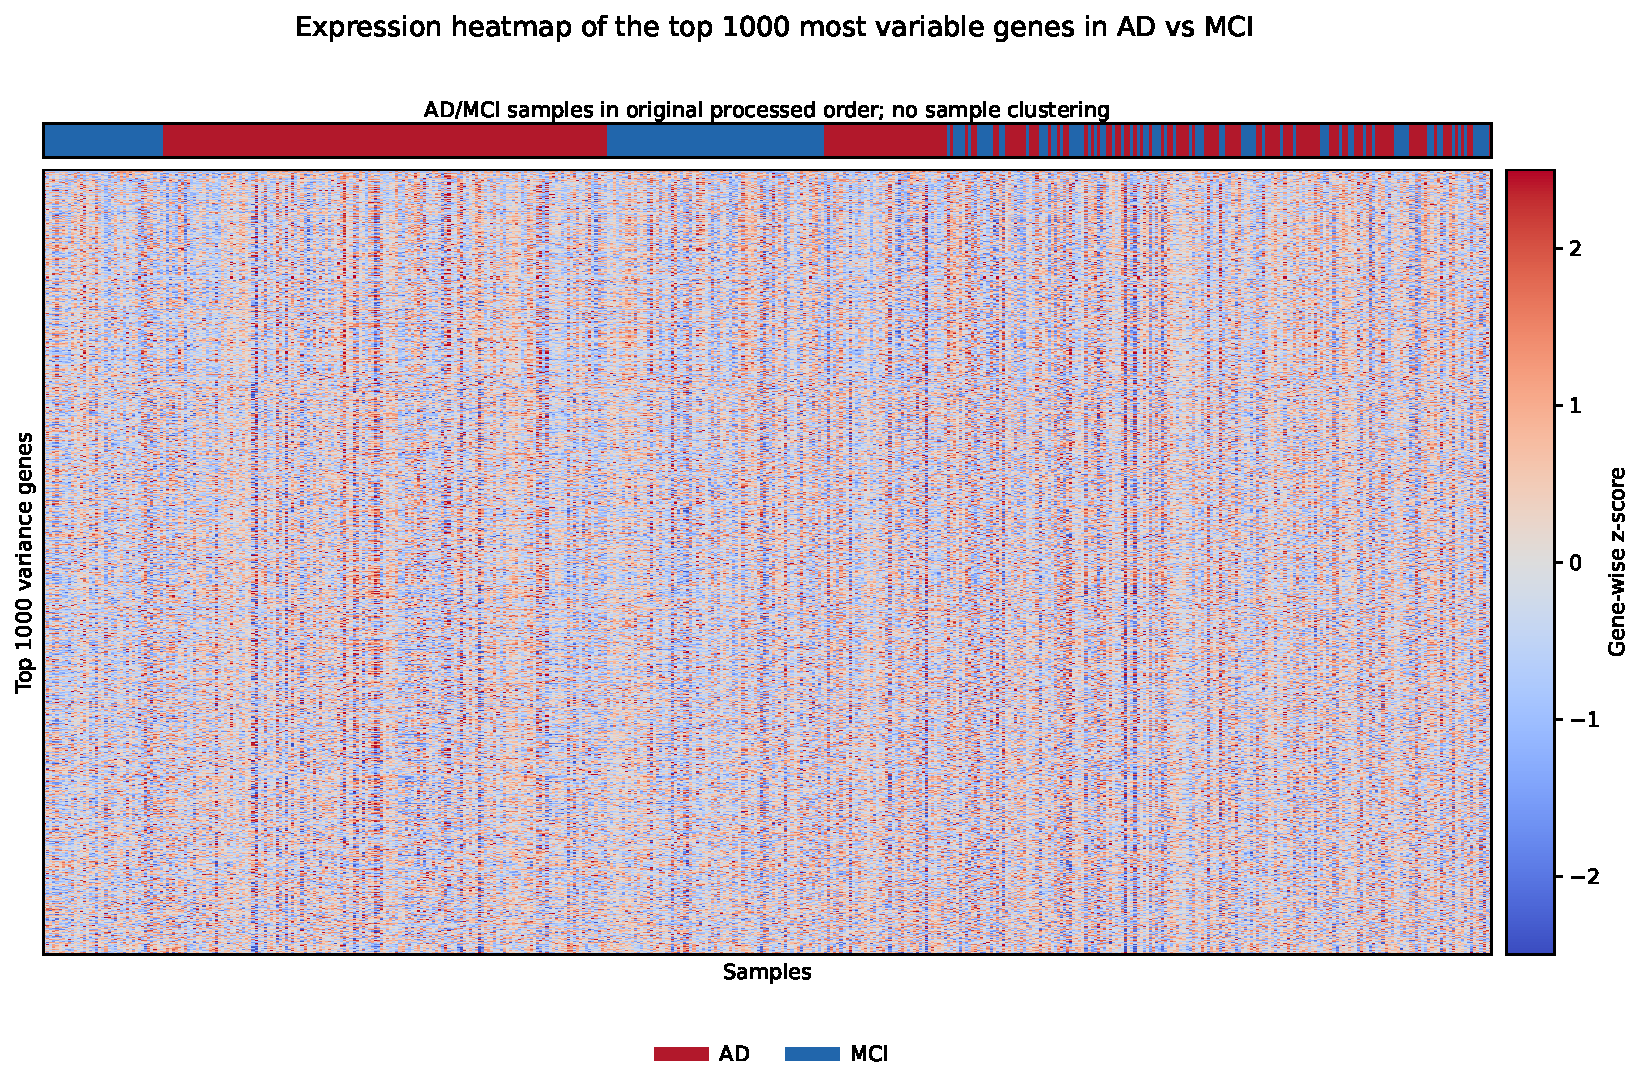
\includegraphics[width=\textwidth]{figures/ch2_heatmap_top1000_variance_ad_mci.pdf}
\caption{Heatmap of the 1000 most variable genes in the AD versus MCI dataset. Expression values are gene-wise standardized and clipped for visualization. Samples are not clustered; the top annotation indicates the clinical label. The absence of clear block structure illustrates the limited separability of AD and MCI from expression values alone.}
\label{fig:ch2-heatmap}
\end{figure}

This figure is descriptive rather than inferential. It does not prove that classification is impossible, and it does not replace a supervised benchmark. Its purpose is to show the geometry of the raw problem. The expression matrix does not provide an obvious visual separation between the two classes. Any useful model must therefore learn subtle distributed patterns rather than exploit a clear class partition visible in the top-variance genes.

The second challenge is class overlap in low-dimensional expression space. Figure~\ref{fig:ch2-pca} shows two-dimensional PCA projections for AD versus MCI and AD versus CTL, again using top-variance expression features. PCA is unsupervised and is not optimized for classification. Nevertheless, it is useful as a diagnostic visualization of global variance structure. In both panels, the classes overlap substantially. The AD versus CTL panel shows a slightly more interpretable trend, while the AD versus MCI panel is highly mixed. This supports the central premise of the thesis: AD versus CTL is a useful reference, but AD versus MCI is the main difficult task.

\begin{figure}[htbp]
\centering
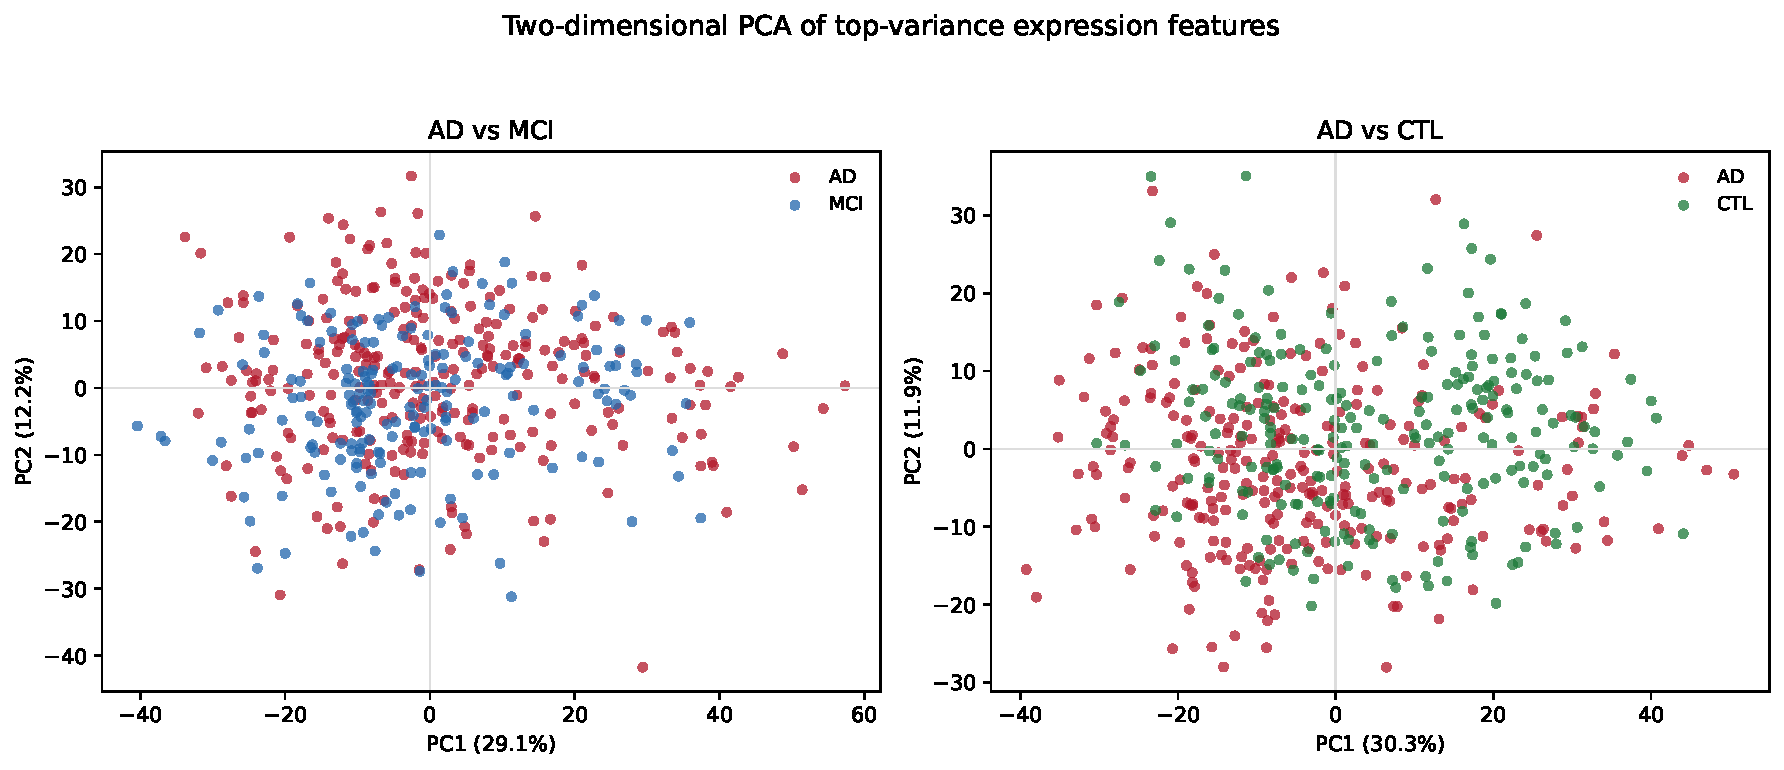
\includegraphics[width=\textwidth]{figures/ch2_pca_ad_mci_ad_ctl.pdf}
\caption{Two-dimensional PCA projections of top-variance expression features for AD versus MCI and AD versus CTL. The projections are unsupervised and are used only to visualize the geometry of the expression space. The strong overlap, especially for AD versus MCI, motivates careful validation and class-balanced metrics.}
\label{fig:ch2-pca}
\end{figure}

The third challenge is high dimensionality. Each subject is described by 19,460 expression features, while the number of samples is in the order of hundreds. This creates many opportunities for spurious associations. Some genes may appear strongly associated with the label only because of the specific split, the batch composition, or random sampling variation. This problem affects both classical machine learning and deep learning. Classical models may overfit through unstable feature selection. Neural models may overfit through excessive capacity relative to the sample size. Regularization and careful validation are therefore necessary, but they are not sufficient unless the entire pipeline is split-aware.

The fourth challenge is feature selection. Reducing the feature space can improve stability and make models easier to train, but feature selection is also one of the most common sources of leakage in transcriptomic studies. If genes are selected using the full dataset before the train-test split, the test labels influence the training pipeline. Even if the final classifier does not directly see the test labels, the feature space has already been optimized using information from the test distribution. This is especially damaging in high-dimensional data, where the number of possible feature subsets is enormous. In this thesis, feature selection is treated as part of the training procedure and must not be fitted on held-out test samples.

The fifth challenge is batch structure. GSE63060 and GSE63061 are related, but they are not technically identical. Batch correction methods such as ComBat can reduce unwanted technical variation \cite{johnson2007combat}, but they can also introduce leakage if fitted on the full dataset before validation. The same issue applies to scaling and normalization parameters. If test samples contribute to the estimation of preprocessing parameters, the evaluation becomes optimistic. Therefore, batch effects are not only a biological or technical nuisance; they are also a validation problem.

The sixth challenge is the biological heterogeneity of MCI. The MCI label includes subjects who may be at different points along the AD continuum and subjects whose impairment may not be AD-related. This means that the MCI class may overlap with both CTL and AD at the molecular level. A model that confuses some MCI subjects with AD may be detecting real disease-stage proximity, or it may simply be failing to separate noisy labels. Without longitudinal follow-up and biomarker confirmation, these possibilities cannot be fully disentangled. This limitation must be kept in mind when interpreting AD/MCI errors.

The final challenge is generalization. A model trained on GSE63060 and GSE63061 may perform well on one split and still fail on a different cohort, platform, or population. Blood gene expression is influenced by age, sex, immune state, medication, sample handling, and many other factors. The thesis therefore avoids presenting model performance as a definitive clinical diagnostic result. Instead, performance is interpreted as evidence about the predictive value and limitations of blood transcriptomic profiles under a controlled experimental protocol. This conservative interpretation is necessary because the main task, AD versus MCI, sits at the intersection of subtle biology, imperfect clinical labels, and high-dimensional machine learning.

\chapter{State of the Art}
\label{ch:state-of-art}

\section{Blood gene expression-based AD classification}
\label{sec:blood-expression-ad-classification}

Blood gene expression has been studied as a possible source of peripheral biomarkers for Alzheimer's disease (AD). The motivation is clear: blood is easier to collect than cerebrospinal fluid, less expensive and more scalable than neuroimaging, and potentially informative about immune, inflammatory, metabolic, and systemic changes associated with neurodegeneration. From a machine learning perspective, blood transcriptomics also provides a high-dimensional molecular representation that can be used for supervised classification.

However, the literature is not centered on the same task addressed in this thesis. Most studies evaluate AD versus cognitively normal controls (CTL or CN). This disease-versus-control setting is useful for showing that blood expression contains some AD-related signal, but it is not equivalent to distinguishing AD dementia from mild cognitive impairment (MCI). The AD/CTL comparison is usually more separable because it contrasts clinically diagnosed dementia with cognitively normal subjects. The AD/MCI comparison is more subtle because MCI is an intermediate and heterogeneous condition. Therefore, a model that performs well on AD versus CTL does not necessarily solve the early-stage problem.

The earliest and most established part of this literature uses classical machine learning or pathway-based models. Voyle et al. \cite{voyle2016pathway} proposed a pathway-based classification approach for AD diagnosis from gene expression. Moradi et al. \cite{moradi2019supervised} later investigated supervised pathway analysis on blood expression profiles. These studies are important because they show that biological structure can be injected into transcriptomic classification, but they are still primarily framed around AD diagnosis rather than AD/MCI separation.

A central reference for this thesis is Lee and Lee \cite{lee2020prediction}. Their study used blood gene expression data from ADNI, GSE63060, and GSE63061 and evaluated several feature representations and machine learning models. Its importance is methodological as much as numerical: the paper explicitly considers cross-cohort generalization, which is essential in blood transcriptomics because platform and batch effects can strongly influence expression profiles. For this reason, the Lee and Lee framework is one of the most relevant baselines reproduced in this thesis.

More recent work has explored deep learning and more complex feature engineering. Kelly et al. \cite{kelly2023blood} studied blood biomarker-based classification for neurodegenerative diseases and evaluated several feature-selection and modelling strategies. Kalkan et al. \cite{kalkan2022image} and Akkaya and Kalkan \cite{akkaya2023one2mfusion} proposed image-based representations of gene expression, where expression vectors are transformed into two-dimensional images and processed with convolutional or fusion models. Jin et al. \cite{jin2023tabnet} used a TabNet-style neural architecture for AD classification from genetic data. Hariharan and Jothi \cite{hariharan2026xai} proposed a more recent deep learning and explainability pipeline with feature selection and augmentation. Sarma and Chatterjee \cite{sarma2025diagnostics} studied stage diagnosis using blood gene expression and clinical data from ADNI.

These studies are relevant, but they are heterogeneous in task definition. Some focus on AD versus CN, some remove MCI samples, some evaluate multiclass CN/MCI/AD classification, and some incorporate clinical variables together with gene expression. Other papers address MCI explicitly, but often in a different way from this thesis. Zhang et al. \cite{zhang2024xgboost} proposed a multiclass XGBoost model and reported pairwise AD/MCI performance, but the primary framing is not a strict binary AD/MCI benchmark. Park et al. \cite{park2024transcriptomics} studied MCI discrimination and conversion to AD, which is closer to prognosis than to cross-sectional AD versus MCI classification. Oh et al. \cite{oh2022neuroinflammation} investigated neuroinflammation-related blood biomarkers across CN, MCI, and AD, with external validation but relatively modest accuracy.

The pattern that emerges is therefore consistent: blood transcriptomic AD classification is active, but direct AD versus MCI classification using only gene expression is much less consolidated than AD versus CTL. Many strong-looking results in the literature are not directly comparable to the main task of this thesis because they solve easier, broader, or differently defined problems. This motivates the structure of the present work: AD versus MCI is treated as the main benchmark, while AD versus CTL is used as a reference task for comparison with published state-of-the-art studies.

\begin{table}[htbp]
\centering
\caption{Task framing in selected blood-transcriptomic AD studies. The main gap for this thesis is the limited number of studies centered directly on transcriptome-only AD versus MCI classification.}
\label{tab:literature-task-framing}
\begin{tabular}{p{0.26\textwidth}p{0.28\textwidth}p{0.36\textwidth}}
\hline
Study family & Main task in the literature & Relevance to this thesis \\
\hline
Pathway and classical ML studies & Mostly AD vs CTL/CN & Useful historical and methodological references \\
Lee and Lee 2020 & AD prediction with cross-cohort evaluation & Strong reference for reproducible AD/CTL benchmarking \\
Image-based and fusion models & Pairwise AD/CN/MCI tasks on pooled data & Relevant but sensitive to feature-engineering leakage \\
TabNet and deep learning studies & AD/CTL or multiclass stage diagnosis & Useful neural baselines, not always AD/MCI-centered \\
MCI conversion studies & Stable/progressive MCI or MCI-to-AD conversion & Clinically related but not identical to cross-sectional AD/MCI \\
\hline
\end{tabular}
\end{table}

\section{Reviewed and reproduced approaches}
\label{sec:reviewed-approaches}

This thesis reproduces or adapts five representative state-of-the-art approaches under a common experimental protocol. The objective is not to replicate every detail of the original studies exactly. Exact replication is often impossible because the papers differ in datasets, preprocessing choices, feature spaces, target definitions, and validation protocols. Instead, the goal is to translate the main methodological ideas of each study into a common local benchmark based on the same processed expression matrices and the same three binary tasks: AD versus MCI, AD versus CTL, and MCI versus CTL.

This design has two advantages. First, it makes the comparison fairer than comparing published numbers taken from different protocols. Second, it directly tests whether methods that are strong in AD versus CTL remain effective in AD versus MCI. This is the critical question for the thesis. If a method performs well only in the easier disease-versus-control setting, its relevance to the main task is limited.

\paragraph{Lee and Lee 2020.}
Lee and Lee \cite{lee2020prediction} is one of the most important references for blood gene expression classification in AD. The study compared several ways of representing the transcriptomic input, including differentially expressed genes, knowledge-driven gene sets, autoencoder or variational autoencoder representations, and hub-gene features. These representations were combined with classifiers such as logistic ridge regression, support vector machines, random forests, and deep neural networks.

The methodological strength of the paper is the attention to cross-cohort evaluation. Blood expression datasets are particularly vulnerable to cohort and platform effects. A method that works only in random cross-validation within a pooled dataset may be learning technical or cohort-specific patterns. Lee and Lee explicitly addressed this issue by evaluating generalization across datasets. For this thesis, the reproduced Lee-style pipeline is used as a strong reference. In the updated local results, the differentially expressed gene representation remains the most competitive Lee and Lee feature set, although the best downstream classifier is task dependent.

\paragraph{Kelly et al. 2023.}
Kelly et al. \cite{kelly2023blood} studied blood biomarker-based classification in a broader neurodegenerative disease context. Their work is relevant because it compares multiple feature-selection strategies and machine learning models, including LASSO, VAE-based reduction, VSSRFE-style feature selection, random forest, SVM, XGBoost, MLP, CNN, and ensemble methods. Although the paper is not designed specifically around AD versus MCI, it represents a modern and systematic benchmark of blood-derived classifiers.

In this thesis, the Kelly-inspired reproduction captures the feature-selection and classifier combinations that can be adapted to the local GEO-based tasks. The most relevant reproduced configuration uses a VSSRFE-LR-style selection with a random forest classifier. This family is important because it represents a more complex feature-selection approach than simple top-variance or DEG filtering, while still remaining in the classical machine learning regime.

\paragraph{One2MFusion 2023.}
Kalkan et al. \cite{kalkan2022image} first proposed an image-based representation of gene expression for AD prediction, and Akkaya and Kalkan \cite{akkaya2023one2mfusion} later extended this direction with One2MFusion. The central idea is to transform gene expression vectors into two-dimensional representations and combine information from the original expression vector and its image representation. This allows convolutional models to be applied to gene expression data, even though the original data are not images.

The approach is interesting because it reports strong pairwise performance in the original paper, including AD/MCI results. However, it is also methodologically delicate. The transformation from gene expression to image representation can involve supervised feature selection, gene ordering, and dimensionality-reduction steps. If these steps are fitted before validation splitting, the reported performance can become optimistic. The reproduction in this thesis evaluates the One2MFusion family under a stricter common protocol, which makes it possible to test how robust the approach remains when leakage is controlled.

\paragraph{Diagnostics 2025.}
Sarma and Chatterjee \cite{sarma2025diagnostics} investigated AD stage diagnosis using blood gene expression and clinical data from ADNI. The paper is relevant because it focuses on multiclass stage diagnosis, considers the high-dimensional low-sample-size nature of gene expression, and evaluates feature selection and augmentation strategies. It also compares gene-expression features with clinical variables, showing that clinical data can dominate performance in some settings.

The original Diagnostics 2025 work is not a direct match for this thesis because it is ADNI-based and multiclass. In this thesis, the gene-expression branch is adapted to the local GEO-based binary tasks. The reproduced pipeline uses an XGBoost/SFBS-inspired feature-selection strategy, optional imbalance handling, and a deep learning classifier. This reproduction is useful because it tests a recent stage-diagnosis strategy under a transcriptome-only, binary benchmark.

\paragraph{Scientific Reports 2026.}
Hariharan and Jothi \cite{hariharan2026xai} proposed a deep learning and explainable AI pipeline for AD prediction from blood gene expression. The study combines feature selection, augmentation, deep neural networks or convolutional models, and post-hoc interpretability. It represents a recent attempt to improve AD prediction with deep learning and XAI-oriented feature analysis.

In the local benchmark, the reproduced version captures the components most compatible with the thesis setting: feature selection, augmentation, and a deep neural classifier. This family is included because it is a recent deep-learning baseline and because it is close in spirit to the thesis motivation of moving beyond simple classical classifiers. At the same time, its performance must be evaluated under the same leakage-aware protocol as the other methods.

Together, these five reproduced families cover a meaningful range of the current literature: classical DEG-based machine learning, systematic feature-selection benchmarks, image-based fusion models, recent stage-diagnosis pipelines, and feature selection with augmentation and deep learning. This range is broad enough to contextualize the proposed Transformer-based model without relying on weak or artificially simple baselines.

\section{Limitations of existing studies for AD versus MCI}
\label{sec:sota-limitations}

The first and most important limitation is task mismatch. A large part of the literature reports AD versus CTL performance. This is not equivalent to AD versus MCI. AD versus CTL compares subjects with diagnosed dementia to cognitively normal controls, while AD versus MCI compares two clinically closer groups. The latter is more relevant to early-stage discrimination and is expected to be more difficult. Therefore, published AD/CTL performance should be treated as a reference, not as a direct state-of-the-art estimate for the main task of this thesis.

The second limitation is that multiclass classification can obscure the specific difficulty of MCI. A CN/MCI/AD classifier may obtain a reasonable overall score while still confusing MCI with AD or CTL. If the main clinical interest is the boundary between MCI and AD, then aggregate multiclass performance is not sufficient. Pairwise AD/MCI evaluation is needed to determine whether the model captures signal specifically at that boundary.

The third limitation is validation heterogeneity. Some studies use external validation across datasets, which is stronger, while others use internal cross-validation on pooled samples. Pooled cross-validation can be problematic when technical batches are present. If samples from GSE63060 and GSE63061 are mixed before splitting, the training and test folds may share dataset-specific structure. This makes performance easier to overestimate. Cross-cohort or batch-aware evaluation is more informative because it tests whether the learned signal survives a distribution shift.

The fourth limitation is leakage from preprocessing and feature selection. Transcriptomic pipelines often include normalization, batch correction, probe filtering, differential expression analysis, gene ranking, dimensionality reduction, augmentation, and model tuning. Each of these steps can leak information if fitted using the full dataset before the validation split. Leakage can be subtle: even if the classifier is trained only on the training set, the feature space itself may already encode information from the test samples. In high-dimensional data, this can have a large effect.

The fifth limitation concerns batch correction. Batch correction is necessary when combining datasets generated under different technical conditions, but it must be performed carefully. Methods such as ComBat \cite{johnson2007combat} estimate batch-related effects from the data. If the held-out test samples are used to estimate these effects during training, the validation protocol is no longer clean. This creates a difficult trade-off: ignoring batch effects can damage generalization, but correcting them incorrectly can create leakage.

The sixth limitation is the use of additional non-transcriptomic information. Some studies include demographic, neuropsychological, or clinical variables together with gene expression. This can be clinically valuable, but it makes the result less comparable to transcriptome-only models. In particular, high performance obtained with cognitive scores or clinical variables cannot be interpreted as evidence that blood gene expression alone is sufficient.

The seventh limitation is metric reporting. Accuracy and ROC-AUC are common, but macro-F1 is reported less consistently. This is a weakness for AD/MCI because the classes are moderately imbalanced and because errors on MCI are especially important. A model with high accuracy may still perform poorly on the MCI class. For this reason, this thesis reports accuracy, macro-F1, and ROC-AUC together, and uses macro-F1 as the main ranking metric for reproduced methods.

These limitations do not make previous work invalid. Rather, they define the conditions under which previous results should be interpreted. The literature shows that blood transcriptomics contains predictive information, especially for AD versus CTL. What remains less clear is how much robust information is available for AD versus MCI under leakage-aware validation. This is the gap that the benchmark in this thesis addresses.

\section{Standardized reproduction protocol}
\label{sec:reproduction-protocol}

Since the reviewed studies were not originally designed for the same task, they were reproduced or adapted under a common protocol. The goal of this protocol is to make the comparison between method families more meaningful. Instead of comparing published scores obtained under different datasets and validation schemes, the reproduced methods are evaluated on the same local datasets and with the same primary metrics.

The input data are the processed gene-level expression matrices derived from GSE63060 and GSE63061. The three tasks are AD versus MCI (473 samples), AD versus CTL (522 samples), and MCI versus CTL (427 samples), each with 19,460 features. The full CTL/MCI/AD cohort is used only as the source from which these binary tasks are derived. The present chapter focuses on binary tasks because they isolate the pairwise comparisons of interest.

All reproduced pipelines follow the same principle: any operation that learns from data must be fitted using the training portion of the split. This includes scaling, feature selection, dimensionality reduction, augmentation, and model training. Test samples are reserved for final evaluation. This principle is especially important for methods that rely on differential expression, LASSO, VSSRFE-style selection, XGBoost ranking, image mapping, or augmentation. These operations can strongly shape the final feature space.

The results reported in this chapter use a common shared-test protocol. For each of ten repetitions, the pooled data are divided into 70\% training, 10\% validation, and 20\% test partitions using the same split manifests for every reproduced method. The present comparison is therefore restricted to within-distribution shared-test performance; cross-dataset transfer results are not included in this section.

All reproducible feature-selection and classifier combinations offered by each adapted approach are evaluated, except for configurations based on all genes. For the descriptive summary, the task-specific configuration with the highest mean shared-test ROC-AUC is reported for each family, with accuracy and macro-F1 taken from the same configuration. Because this is a test-summary selection rather than a nested model-comparison procedure, the selected values are interpreted as exploratory upper envelopes.

The five reproduced families included in the updated comparison are:
\begin{itemize}
    \item a Lee and Lee 2020-inspired DEG and classical machine learning pipeline;
    \item a Kelly et al. 2023-inspired feature-selection and random forest pipeline;
    \item a One2MFusion-inspired vector/image fusion pipeline;
    \item a Diagnostics 2025-inspired feature-selection, imbalance-handling, and deep learning pipeline;
    \item a Scientific Reports 2026-inspired feature-selection, augmentation, and deep learning pipeline.
\end{itemize}

The proposed TxT configuration is considered separately in the following chapters and is therefore not included in the tables of reproduced approaches.

\section{Results of the reproduced approaches}
\label{sec:sota-results}

This section reports the updated shared-test results of the five approaches reproduced from the literature. TxT is considered separately in the following chapters, so that the reproduced reference methods can first be examined on their own.

\paragraph{Reporting rule.}
All reproducible combinations of feature-selection method and classifier offered by each adapted approach were evaluated on the same split manifests. The data were divided into 70\% training, 10\% validation, and 20\% test partitions, and the experiment was repeated ten times. All transformations learned from the data, including scaling, feature selection, dimensionality reduction, augmentation, and model fitting, were restricted to the training partition. Configurations based on all genes were excluded from both model selection and reporting.

Rather than fixing one arbitrary configuration for each study across all tasks, the tables report the task-specific configuration with the highest mean shared-test ROC-AUC within each reproduced family. Accuracy and macro-F1 are taken from that same configuration. Consequently, each row is an exploratory upper envelope over the configurations evaluated for that family, not a post-selection estimate from a nested model-comparison procedure. Values are reported as mean \(\pm\) standard deviation across repeats, and bold type marks the best mean for each metric within a task.

\subsection*{AD versus MCI}

\begin{table}[htbp]
\centering
\begingroup
\footnotesize
\renewcommand{\arraystretch}{1.35}
\setlength{\tabcolsep}{3.5pt}
\begin{tabularx}{\textwidth}{
    >{\raggedright\arraybackslash}p{0.18\textwidth}
    >{\raggedright\arraybackslash}X
    >{\centering\arraybackslash}p{0.15\textwidth}
    >{\centering\arraybackslash}p{0.15\textwidth}
    >{\centering\arraybackslash}p{0.15\textwidth}
}
\toprule
\rowcolor{gray!18}
\textbf{Reference} &
\textbf{Selected configuration} &
\textbf{Accuracy} &
\textbf{Macro-F1} &
\textbf{ROC-AUC} \\
\midrule

\textbf{Lee and Lee 2020}\textsuperscript{\(\dagger\)} &
DEG + logistic regression &
\(0.584 \pm 0.053\) &
\(0.533 \pm 0.056\) &
\(0.596 \pm 0.045\) \\

\rowcolor{gray!5}
\textbf{Kelly et al. 2023} &
VSSRFE--LR + random forest &
\(\mathbf{0.614 \pm 0.013}\) &
\(0.505 \pm 0.028\) &
\(0.612 \pm 0.059\) \\

\textbf{One2MFusion 2023} &
CNN branch &
\(0.591 \pm 0.039\) &
\(0.527 \pm 0.088\) &
\(0.616 \pm 0.038\) \\

\rowcolor{gray!5}
\textbf{Diagnostics 2025} &
XGBoost/SFBS + Borderline-SMOTE + random forest &
\(0.600 \pm 0.042\) &
\(0.551 \pm 0.049\) &
\(0.607 \pm 0.046\) \\

\textbf{Hariharan and Jothi 2026} &
RFE + SVM, without augmentation &
\(0.605 \pm 0.039\) &
\(\mathbf{0.598 \pm 0.036}\) &
\(\mathbf{0.657 \pm 0.050}\) \\

\bottomrule
\end{tabularx}
\endgroup
\caption{Shared-test results on AD versus MCI. The reported configuration maximizes mean ROC-AUC within each reproduced family after excluding all-gene variants. All rows use ten repeats except Lee and Lee\textsuperscript{\(\dagger\)}, which uses six valid repeats.}
\label{tab:ad-mci-sota-results}
\end{table}

The Lee and Lee estimate is based on six valid repeats rather than ten. In repeats 6, 8, 9, and 10, train-only limma selection returned no genes at the prespecified adjusted-\(p<0.01\) threshold; no fallback genes were introduced. This row is therefore incomplete and should not be compared with the ten-repeat estimates as if it had the same precision.

AD versus MCI remains the most difficult task. The highest mean ROC-AUC is obtained by the Hariharan and Jothi reproduction using unaugmented RFE features and an SVM (\(0.657\)), which also gives the best macro-F1 (\(0.598\)). Kelly et al. yields the highest accuracy (\(0.614\)), but its lower macro-F1 (\(0.505\)) indicates less balanced thresholded predictions. One2MFusion's strongest variant is the standalone CNN branch rather than the full fusion model, while the best Diagnostics variant replaces the originally emphasized dense network with a random forest. These changes illustrate why evaluating the complete reproducible model matrix is more informative than retaining a single hand-picked configuration.

\subsection*{AD versus CTL}

\begin{table}[htbp]
\centering
\begingroup
\footnotesize
\renewcommand{\arraystretch}{1.35}
\setlength{\tabcolsep}{3.5pt}
\begin{tabularx}{\textwidth}{
    >{\raggedright\arraybackslash}p{0.18\textwidth}
    >{\raggedright\arraybackslash}X
    >{\centering\arraybackslash}p{0.15\textwidth}
    >{\centering\arraybackslash}p{0.15\textwidth}
    >{\centering\arraybackslash}p{0.15\textwidth}
}
\toprule
\rowcolor{gray!18}
\textbf{Reference} &
\textbf{Selected configuration} &
\textbf{Accuracy} &
\textbf{Macro-F1} &
\textbf{ROC-AUC} \\
\midrule

\textbf{Lee and Lee 2020} &
DEG + dense neural network &
\(0.733 \pm 0.035\) &
\(0.724 \pm 0.042\) &
\(0.834 \pm 0.025\) \\

\rowcolor{gray!5}
\textbf{Kelly et al. 2023} &
VSSRFE--LR + random forest &
\(0.737 \pm 0.044\) &
\(0.734 \pm 0.045\) &
\(\mathbf{0.848 \pm 0.027}\) \\

\textbf{One2MFusion 2023} &
FNN/CNN fusion &
\(0.710 \pm 0.032\) &
\(0.689 \pm 0.043\) &
\(0.812 \pm 0.030\) \\

\rowcolor{gray!5}
\textbf{Diagnostics 2025} &
XGBoost/SFBS + Borderline-SMOTE + random forest &
\(\mathbf{0.749 \pm 0.025}\) &
\(\mathbf{0.745 \pm 0.027}\) &
\(0.836 \pm 0.031\) \\

\textbf{Hariharan and Jothi 2026} &
RFE + SVM, without augmentation &
\(0.727 \pm 0.033\) &
\(0.724 \pm 0.033\) &
\(0.810 \pm 0.027\) \\

\bottomrule
\end{tabularx}
\endgroup
\caption{Shared-test results on AD versus CTL over ten repetitions. The reported configuration maximizes mean ROC-AUC within each reproduced family after excluding all-gene variants.}
\label{tab:ad-ctl-sota-results}
\end{table}

Performance is consistently higher on AD versus CTL. Kelly et al. provides the strongest ranking performance, with a mean ROC-AUC of \(0.848\). Diagnostics provides the highest accuracy (\(0.749\)) and macro-F1 (\(0.745\)), while its ROC-AUC of \(0.836\) is close to those of Kelly et al. and Lee and Lee. The two image or deep-learning-oriented families also exceed \(0.80\) ROC-AUC, but neither improves on the strongest classical combinations.

\subsection*{MCI versus CTL}

\begin{table}[htbp]
\centering
\begingroup
\footnotesize
\renewcommand{\arraystretch}{1.35}
\setlength{\tabcolsep}{3.5pt}
\begin{tabularx}{\textwidth}{
    >{\raggedright\arraybackslash}p{0.18\textwidth}
    >{\raggedright\arraybackslash}X
    >{\centering\arraybackslash}p{0.15\textwidth}
    >{\centering\arraybackslash}p{0.15\textwidth}
    >{\centering\arraybackslash}p{0.15\textwidth}
}
\toprule
\rowcolor{gray!18}
\textbf{Reference} &
\textbf{Selected configuration} &
\textbf{Accuracy} &
\textbf{Macro-F1} &
\textbf{ROC-AUC} \\
\midrule

\textbf{Lee and Lee 2020} &
DEG + dense neural network &
\(0.695 \pm 0.075\) &
\(0.684 \pm 0.083\) &
\(\mathbf{0.782 \pm 0.059}\) \\

\rowcolor{gray!5}
\textbf{Kelly et al. 2023} &
VSSRFE--LR + random forest &
\(\mathbf{0.723 \pm 0.053}\) &
\(\mathbf{0.714 \pm 0.054}\) &
\(0.777 \pm 0.052\) \\

\textbf{One2MFusion 2023} &
FNN/CNN fusion &
\(0.672 \pm 0.066\) &
\(0.651 \pm 0.087\) &
\(0.742 \pm 0.071\) \\

\rowcolor{gray!5}
\textbf{Diagnostics 2025} &
XGBoost/SFBS + random forest, without SMOTE &
\(0.708 \pm 0.072\) &
\(0.700 \pm 0.071\) &
\(0.770 \pm 0.058\) \\

\textbf{Hariharan and Jothi 2026} &
Chi-square + SVM, without augmentation &
\(0.672 \pm 0.062\) &
\(0.671 \pm 0.062\) &
\(0.742 \pm 0.058\) \\

\bottomrule
\end{tabularx}
\endgroup
\caption{Shared-test results on MCI versus CTL over ten repetitions. The reported configuration maximizes mean ROC-AUC within each reproduced family after excluding all-gene variants.}
\label{tab:mci-ctl-sota-results}
\end{table}

MCI versus CTL occupies an intermediate position between the other two tasks. Lee and Lee obtains the highest mean ROC-AUC (\(0.782\)), whereas Kelly et al. gives the strongest thresholded performance, with accuracy \(0.723\) and macro-F1 \(0.714\). Diagnostics is close to both methods. One2MFusion and Hariharan and Jothi reach the same rounded ROC-AUC (\(0.742\)), although the Hariharan and Jothi configuration gives the more balanced macro-F1.

\medskip
Across the three tasks, the best mean ROC-AUC decreases from \(0.848\) for AD versus CTL to \(0.782\) for MCI versus CTL and \(0.657\) for AD versus MCI. The corresponding best macro-F1 values are \(0.745\), \(0.714\), and \(0.598\). This ordering is consistent with the increasing clinical similarity of the compared groups and confirms that strong AD-versus-control performance does not imply equally strong discrimination between AD and MCI.

The updated results also weaken any simple claim that greater architectural complexity is beneficial. Nine of the fifteen reported family-by-task configurations use either a random forest or an SVM after explicit feature selection; the full One2MFusion model is selected only for the two control comparisons. For the Hariharan and Jothi reproduction, the selected ten-repeat configurations are unaugmented. The separate three-repeat CTGAN pilot is not included in the main tables because it does not provide an estimate with the same repetition count.

These observations are descriptive. No formal statistical test was conducted, several differences are small relative to their between-repeat standard deviations, and the task-specific configurations were identified from the shared-test summaries. The reported values should therefore not be interpreted as confirmatory evidence that one method is superior. They describe the performance range observed for the reproduced approaches under the common leakage-aware protocol, using only selected-gene representations and the same repeated shared-test partitions.



% Suggested bibliography command in the full thesis file:
% \bibliographystyle{apalike}
% \bibliography{references_chapter1,references_chapter2_3}
